\documentclass{article}

\usepackage{graphicx}
\usepackage{tikz}
\usepackage{tikzsymbols}
\usetikzlibrary{calc,patterns,shapes.geometric}
\pagestyle{empty}
\usepackage[margin=0pt]{geometry}
\geometry{papersize={14in,12in}}

\def\centerarc[#1](#2)(#3:#4:#5){\draw[#1] ($(#2)+({#5*cos(#3)},{#5*sin(#3)})$) arc (#3:#4:#5);}

\begin{document}
	\begin{figure}
		\centering
		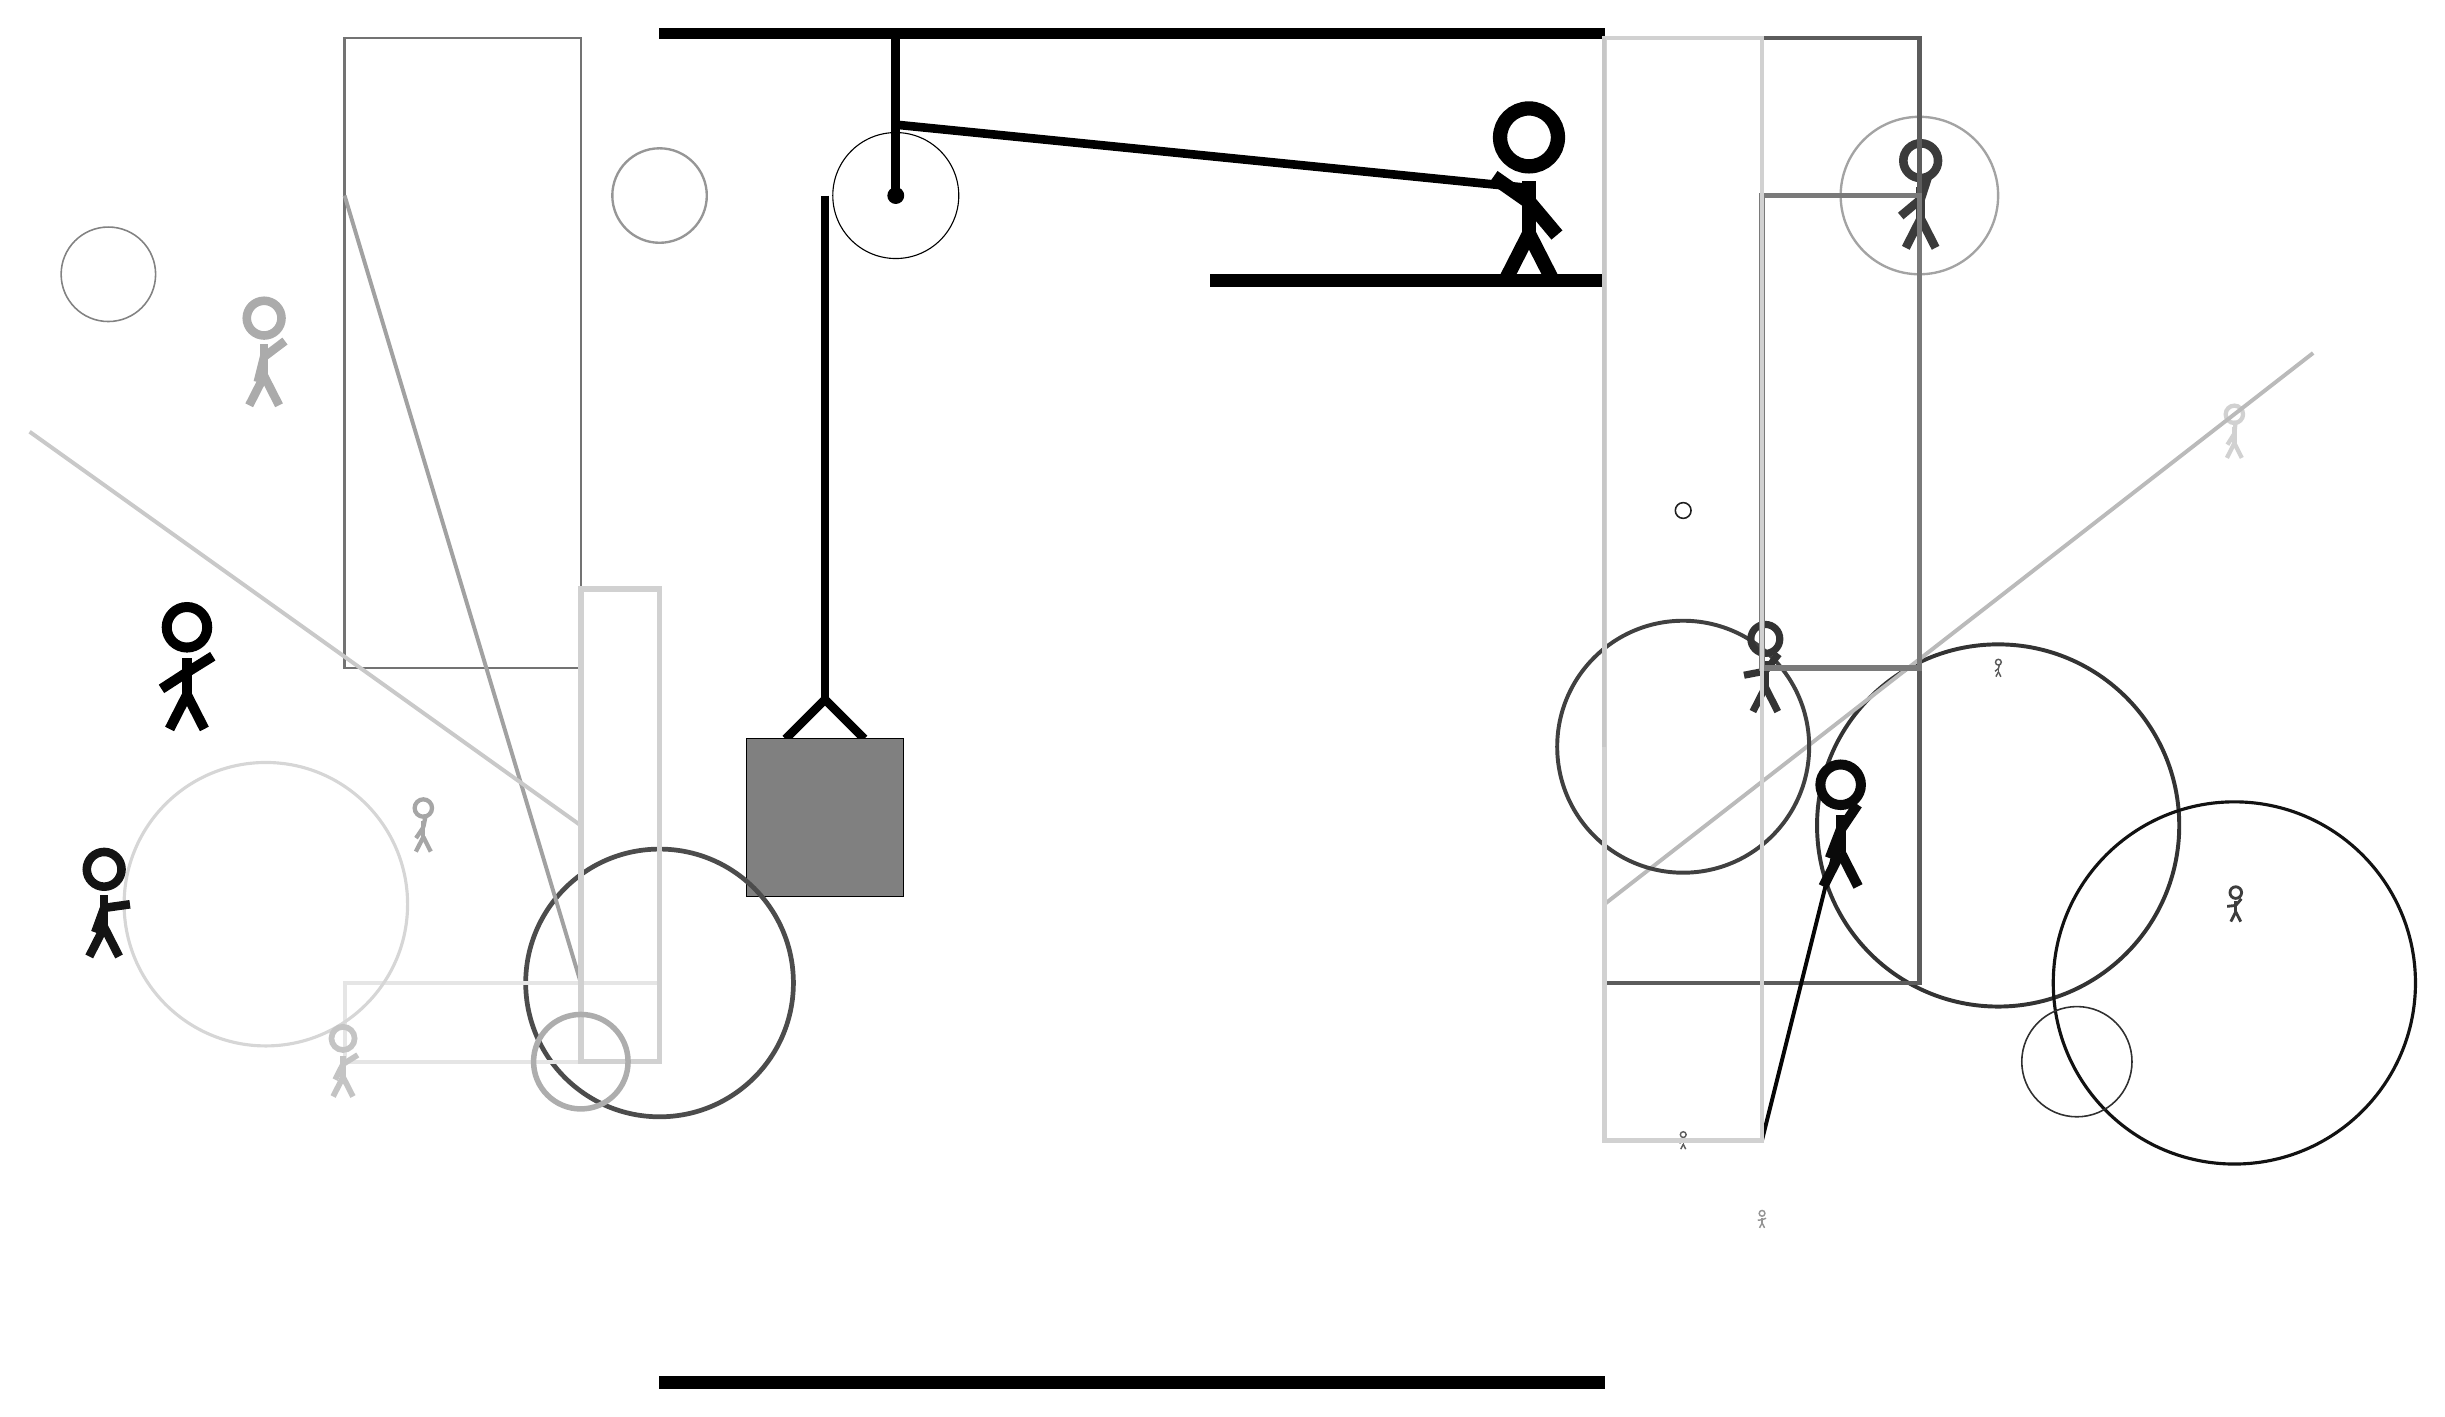
\begin{tikzpicture}
			%%%%% START %%%%%
			
			\draw[fill=black] (-2, 14) rectangle (10, 14.125);
			
			\draw (1, 12) circle (0.8);
			\draw[fill=black] (1, 12) circle (0.1);
			\draw[line width=1.1mm] (1, 14) -- (1, 12);
			
			\draw[line width=1.1mm](-0.4, 5.1) --  (0.1, 5.6) -- (0.6, 5.1);
			\draw[fill=black!50] (-0.9, 5.1) rectangle (1.1, 3.1);
			
			\draw[line width=1.1mm](0.1, 12) -- (0.1, 5.6);
			\centerarc[line width=1.1mm](1, 12)(90:180:0.9)
			\draw[line width=1.1mm](1, 12.9) -- (9, 12.1);
			
			\node at (9, 12) {\Strichmaxerl[10][-35][-50]};
			\draw[fill=black] (5, 11) rectangle (10, 10.85);
			
			\node[line width=0.7mm, color=black!35] at (-5, 4) {\Strichmaxerl[3][56][79]};
			
			\draw [line width=0.2mm, color=black!49](-9, 11) circle (0.6);
			\draw [line width=0.6mm, color=black!70](-2, 2) circle (1.7);
			\node[line width=0.3mm, color=black!77] at (14, 12) {\Strichmaxerl[6][40][72]};
			\draw [line width=0.3mm, color=black!36](14, 12) circle (1.0);
			\draw[line width=0.3mm, color=black!55] (-3, 14) rectangle (-6, 6);
			\draw[line width=0.5mm, color=black!10] (-2, 2) rectangle (-6, 1);
			\draw [line width=0.5mm, color=black!80](15, 4) circle (2.3);
			\node[line width=0.2mm, color=black!18] at (18, 9) {\Strichmaxerl[3][58][84]};
			\draw [line width=0.4mm, color=black!16](-7, 3) circle (1.8);
			\draw [line width=0.4mm, color=black!93](18, 2) circle (2.3);
			\draw[line width=0.5mm, color=black!37](-3, 2) -- (-6, 12);
			\draw [line width=0.2mm, color=black!81](16, 1) circle (0.7);
			
			\draw[line width=0.6mm, color=black!64] (10, 14) rectangle (14, 2);
			\node[line width=0.6mm, color=black!92] at (-9, 3) {\Strichmaxerl[6][70][8]};
			\node[line width=0.3mm, color=black!33] at (-7, 10) {\Strichmaxerl[6][76][37]};
			\draw[line width=0.5mm, color=black!27](10, 3) -- (19, 10);
			\node[line width=0.2mm, color=black!65] at (15, 6) {\Strichmaxerl[1][38][75]};
			\node[line width=0.3mm, color=black!63] at (11, 0) {\Strichmaxerl[1][30][33]};
			
			\draw [line width=0.7mm, color=black!68](-5, 11) circle (0.0);
			\node[line width=0.6mm, color=black!76] at (18, 3) {\Strichmaxerl[2][6][50]};
			\node[line width=0.7mm, color=black!100] at (-8, 6) {\Strichmaxerl[7][33][32]};
			\draw[line width=0.5mm, color=black!98](12, 0) -- (13, 4);
			\draw [line width=0.3mm, color=black!41](-2, 12) circle (0.6);
			\draw [line width=0.5mm, color=black!75](11, 5) circle (1.6);
			
			\draw[line width=0.5mm, color=black!21](-3, 4) -- (-10, 9);
			
			\node[line width=0.6mm, color=black!23] at (-6, 1) {\Strichmaxerl[4][63][32]};
			\node[line width=0.3mm, color=black!80] at (12, 6) {\Strichmaxerl[5][11][52]};
			
			\draw [line width=0.2mm, color=black!88](11, 8) circle (0.1);
			\node[line width=0.7mm, color=black!96] at (13, 4) {\Strichmaxerl[7][69][56]};
			\draw[line width=0.7mm, color=black!52] (12, 12) rectangle (14, 6);
			\node[line width=0.5mm, color=black!42] at (12, -1) {\Strichmaxerl[1][6][22]};
			\draw[line width=0.6mm, color=black!18] (12, 0) rectangle (10, 14);
			\draw[line width=0.7mm, color=black!18] (-3, 1) rectangle (-2, 7);
			\draw [line width=0.7mm, color=black!32](-3, 1) circle (0.6);
			\draw[line width=0.5mm, color=black!22](10, 14) -- (10, 5);
			
			\draw[fill=black] (-2, -3) rectangle (10, -3.15);
			
			%%%%% END %%%%%
		\end{tikzpicture}
	\end{figure}	
\end{document}